\documentclass[fleqn,answers,addpoints]{exam}

%\usepackage{graphicx, fancyhdr}
\usepackage{etoolbox}
\usepackage{subcaption}
\usepackage{etoolbox}
\usepackage{tikz,pgfplots}
\usepackage{amsmath, amsfonts}
\usepackage{color}

%% For LaTeX-Box: root = stat105_exam1_info.tex 
%%%%%%%%%%%%%%%%%%%%%%%%%%%%%%%%%%%%%%%%%%%%%%%%%%%%%%%%%%%%%%%%%%%%%%%%%%%%%%%%
%  File Name: stat105_exam1_info.tex
%  Purpose:
%
%  Creation Date: 24-09-2015
%  Last Modified: Thu Sep 24 13:51:36 2015
%  Created By:
%%%%%%%%%%%%%%%%%%%%%%%%%%%%%%%%%%%%%%%%%%%%%%%%%%%%%%%%%%%%%%%%%%%%%%%%%%%%%%%%
\newcommand{\course}[1]{\ifstrempty{#1}{STAT 105}{STAT 105, Section #1}}
\newcommand{\sectionNumber}{B}
\newcommand{\examDate}{October 1, 2015}
\newcommand{\semester}{FALL 2015}
\newcommand{\examNumber}{II}

\newcommand{\examTitle}{Exam \examNumber}

\runningheader{\course{\sectionNumber}}{Exam \examNumber}{\examDate}
\runningfooter{}{}{Page \thepage of \numpages}

\newcommand{\examCoverPage}{
   \begin{coverpages}
   \centering
   {\bfseries\scshape\Huge Exam I \par}
   \vspace{1cm}
   {\bfseries\scshape\LARGE \course{\sectionNumber} \par}
   {\bfseries\scshape\LARGE \semester \par}

   \vspace{2cm}

   \fbox{\fbox{\parbox{5.5in}{\centering 

      \vspace{.25cm} 
      
      {\bfseries\Large Instructions} \\

      \vspace{.5cm} 

      \begin{itemize}
         \item  The exam is scheduled for 80 minutes, from 8:00 to 9:20 AM. At 9:20 AM the exam will end.\\
         \item  A forumula sheet is attached to the end of the exam. Feel free to tear it off.\\
         \item  You may use a calculator during this exam.\\
         \item  Answer the questions in the space provided. If you run out of room, continue on the back of the page. \\
         \item  If you have any questions about, or need clarification on the meaning of an item on this exam, please ask your instructor. No other form of external help is permitted attempting to receive help or provide help to others will be considered cheating.\\
         \item  {\bfseries Do not cheat on this exam.} Academic integrity demands an honest and fair testing environment. Cheating will not be tolerated and will result in an immediate score of 0 on the exam and an incident report will be submitted to the dean's office.\\
      \end{itemize}

   }}}

   \vspace{2cm}

   \makebox[0.6\textwidth]{Name:\enspace\hrulefill}

   \vspace{1cm}

   \makebox[0.6\textwidth]{Student ID:\enspace\hrulefill}
   \end{coverpages}

}


\newcommand{\course}[1]{\ifstrempty{#1}{STAT 305}{STAT 305, Section #1}}
\newcommand{\sectionNumber}{B}
\newcommand{\examDate}{April 11, 2019}
\newcommand{\semester}{Spring 2019}
\newcommand{\examNumber}{II}
\newcommand{\qparts}[1]{\begin{parts} #1 \end{parts}}

% Document definitions
\newcommand{\examTitle}{Exam \examNumber}
\runningheader{\course{\sectionNumber}}{Exam \examNumber}{\examDate}
\runningfooter{}{}{Page\ \thepage\ of\ \numpages}

\begin{document}

\begin{coverpages}
   \centering
   {\bfseries\scshape\Huge Exam \examNumber \par}
   \vspace{1cm}
   {\bfseries\scshape\LARGE \course{\sectionNumber} \par}
   {\bfseries\scshape\LARGE \semester \par}
   \vspace{2cm}
   \fbox{\fbox{\parbox{5.5in}{
      \centering 
      \vspace{.25cm} 
      {\bfseries\Large Instructions} \\
      \vspace{.25cm} 
      \begin{itemize}
         \item  The exam is scheduled for 80 minutes, from 3:40 to 5:00 PM. At 5:00 PM the exam will end.\\
         \item  A forumula sheet is attached to the end of the exam. Feel free to tear it off.\\
         \item  You are allowed to use a self-produced one-page (front and back) formula sheet during this exam.\\
         \item  You may use a calculator during this exam.\\
         \item  Answer the questions in the space provided. If you run out of room, continue on the back of the page. \\
         \item  If you have any questions about, or need clarification on the meaning of an item on this exam, please ask your instructor. No other form of external help is permitted attempting to receive help or provide help to others will be considered cheating.\\
         \item  {\bfseries Do not cheat on this exam.} Academic integrity demands an honest and fair testing environment. Cheating will not be tolerated and will result in an immediate score of 0 on the exam and an incident report will be submitted to the office of the dean.\\
      \end{itemize}
   }}}
   \vspace{1cm}
   \makebox[0.6\textwidth]{}
   \vspace{1cm}
   \makebox[0.6\textwidth]{Name:\enspace\hrulefill}
   \vspace{1cm}
   \makebox[0.6\textwidth]{Student ID:\enspace\hrulefill}
\end{coverpages}

\begin{questions}

\question[2] For discrete distributions, the probability function is
\fillin~and the cumulative probability function is \fillin.

\begin{oneparchoices}
\choice discontinuous and discontinuous
\choice discontinuous and continuous
\choice continuous and continuous
\choice continuous and discontinuous
\end{oneparchoices}
\vspace{1cm}

\question[3]Circle the name of the distribution which best matches the
plot of the probability density function:

\begin{center}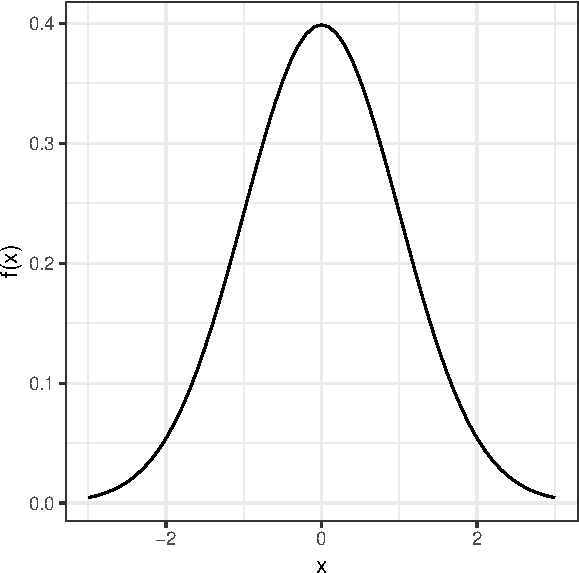
\includegraphics[width=.4\linewidth,height=.4\linewidth]{stat305-exam2_files/figure-latex/unnamed-chunk-2-1} \end{center}
\begin{oneparchoices}
\choice exponential 
\choice normal 
\choice uniform
\choice binomial
\end{oneparchoices}
\vspace{1cm}

\question[3]Circle the name of the distribution which best matches the
plot of the cumulative density function:

\begin{center}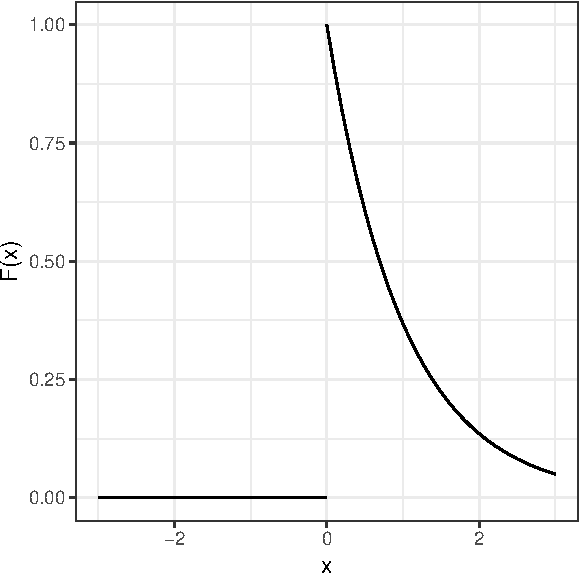
\includegraphics[width=.4\linewidth,height=.4\linewidth]{stat305-exam2_files/figure-latex/unnamed-chunk-3-1} \end{center}
\begin{oneparchoices}
\choice exponential 
\choice normal 
\choice uniform
\choice binomial
\end{oneparchoices}

\newpage

\question[4] The left plot depicts the probability density function of a
step-uniform random variable. In the plot on the right, sketch the
corresponding cumulative density function.

\begin{center}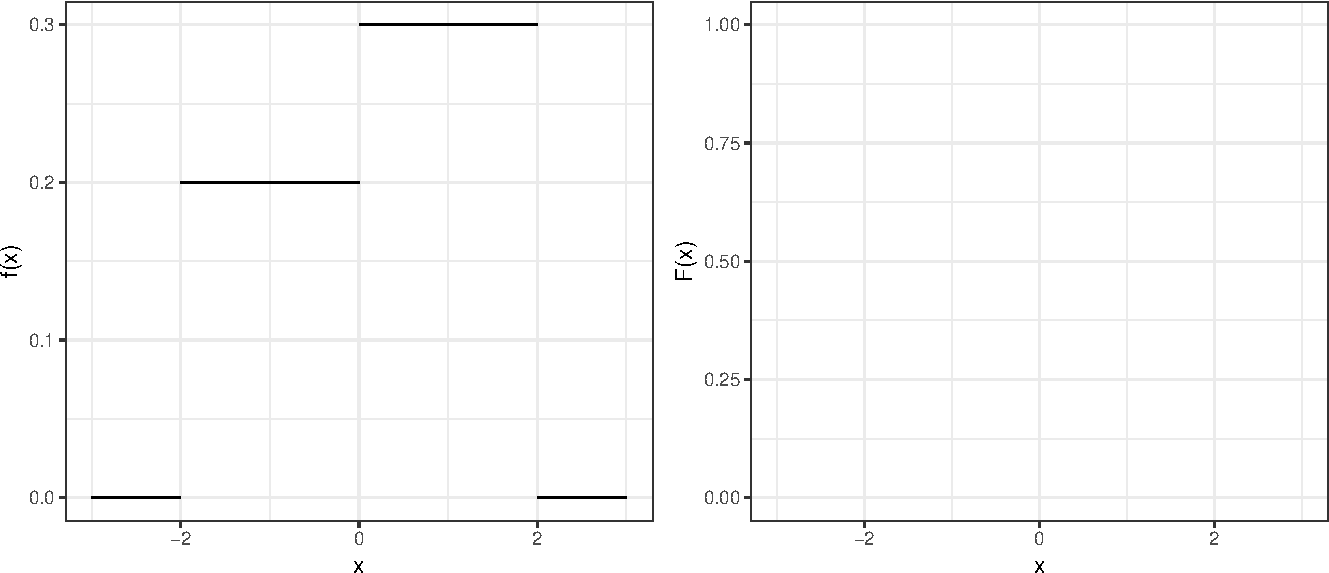
\includegraphics[width=0.9\linewidth,height=.4\linewidth]{stat305-exam2_files/figure-latex/unnamed-chunk-4-1} \end{center}

\vspace{1cm}

\question Suppose \(X\) is a discrete random variable with following
probability function:
\[ f(x) = \begin{cases} 0.1 & x = -2, 0, 2 \\ 0.35 & x = -1, 1 \\ 0 & o.w. \end{cases} \]

\qparts{
\part[2] Find $P(X = 0)$ \vspace{2.5cm}
\part[2] Find $P(X \le 0)$ \vspace{2.5cm}
\part[2] Find $P(X \ne 0)$ \vspace{2.5cm}
}

\newpage

\question

Two manufacturers (A and B) of the same electrical circuit board are
being used by a company. The boards have five circuit connectors which
can either be defective or non-defective (meaning that each circuit
board could have 0, 1, 2, 3, 4, or 5 nondefective connectors). The
company knows that the manufacturer matters when it comes to the chance
that the connectors are defective. Unfortunately, all the circuit boards
have been placed in the same container and there is no clear way to tell
them apart. We do know the following though:
\[P(\text{``There are }k\text{ defective connectors on the board"} | \text{``The board is manufacturer A"}) = \frac{5!}{(5-k)! k!} \left(\frac{1}{4}\right)^k \left(\frac{3}{4}\right)^{5 - k} \]\\
\[P(\text{``There are }k\text{ defective connectors on the board"} | \text{``The board is manufacturer B"}) = \frac{5!}{(5-k)! k!} \left(\frac{1}{2}\right)^k \left(\frac{1}{2}\right)^{5 - k} \]\\
Suppose that we also know that there were 300 boards of manufacturer A
and 200 boards of manufacturer B.

\qparts{
\part[2] Find the probability that a randomly chosen board is from manufacturer A. \vspace{3cm}
\part[2] Find the probability that a randomly chosen board has no defective connectors \textit{given} that it is from manufacturer A. \vspace{3cm}
\part[2] Find the probability that a randomly chosen board is from manufacturer A and has 0 defective connectors. \vspace{3cm}
\part[2] Find the probability that a randomly chosen board is from manufacturer B and has 0 defective connectors. \vspace{3cm}
\part[2] Find the probability that a randomly chosen board has 0 defective connectors. \vspace{3cm}
\part[2] Find the probability that a randomly chosen board is from manufacturer A \textit{given} that it has 0 defective connectors. \vspace{5cm}
\part[2] Find the probability that a randomly chosen board is from manufacturer B \textit{given} that it has 2 defective connectors. \vspace{5cm}
}

\newpage

\question

Let \(X\) be a poisson random variable with \(\lambda = 6\). \qparts{
\part[2] Find $P(X = 3)$ \vspace{2cm}
\part[2] Find $P(X < 2)$ \vspace{2cm}
\part[2] Find $E(X)$ \vspace{2cm}
\part[2] Find $Var(X)$ \vspace{2cm}
}

\question

Let \(Y\) be an exponential random variable with mean 2. \qparts{
\part[2] Find $P(Y \le 3)$ \vspace{2cm}
\part[2] Find $P(1 \le Y \le 3)$ \vspace{3cm}
\part[2] Find $E(Y)$ \vspace{2cm}
\part[2] Find $Var(Y)$ \vspace{2cm}
}

\newpage

\question

Let \(X\) be a normal random variable with a mean of 2 and a varaince of
9 (i.e., \(X \sim N(2,9)\)) and let \(Z\) be a random variable following
a standard normal distribution. Find the following probabilities (note:
Table B-3 will be helpful): \vspace{1cm} \qparts{
  \part[2] $P(Z \le 2)$ \vspace{2cm}
  \part[2] $P(|Z| \ge 1)$ \vspace{2cm}
  \part[2] $P(0 \le Z < 3)$ \vspace{2cm}
  \part[2] $P(X < 3)$ \vspace{3cm}
  \part[2] $P(|X-2| \le 2.5)$ \vspace{3cm}
  \part[5] Find the value $a$ so that $P(X < a) = .95$ (hint: start with a standard normal)
}

\newpage

\question

Suppose that \(X\) is a continuous random variable with probability
density function (pdf):
\[ f(x) = \begin{cases} 0.25 + c x^2 &  -1 < x < 1 \\ 0 & \text{otherwise} \end{cases} \]
where \(c\) is a constant (not necessarily positive).

\qparts{
\part[2] What is the value of $c$ if $f(x)$ is a valid probability density function? \vspace{2cm}
\part[5] Sketch the probability density function using the grid below (including the points $(-1, f(1))$, $(0, f(0))$, and $(1, f(1))$).


\begin{center}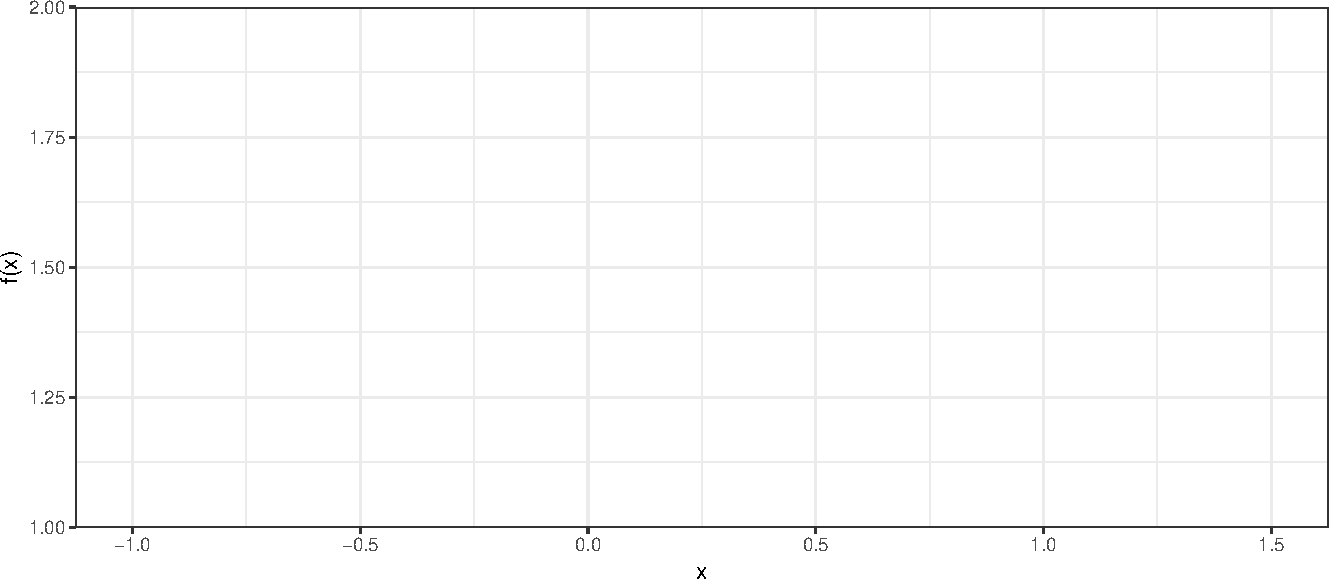
\includegraphics[width=0.9\linewidth,height=.4\linewidth]{stat305-exam2_files/figure-latex/unnamed-chunk-5-1} \end{center}
\part[4] What is the cumulative density function, $F(x)$? \vspace{3cm}
\part[2] What is the probability that $X$ takes a value greater than 1? \vspace{2cm}
\part[2] What is the probability that $X$ takes a value between 0 and 1? \vspace{2cm}
}

\end{questions}

\end{document}
